\section{Text to Schema}

The task of translating natural-language requirement descriptions into a logical relational schema differs fundamentally from the more widely studied problem of natural-language-to-query translation (Text\textrightarrow SQL). In the Text\textrightarrow SQL literature, the database schema is typically assumed to be predefined, stable, and correct; learning and inference methods are therefore explicitly conditioned on existing table structures, column names, and foreign-key relationships when mapping user utterances to executable queries. By contrast, the Text\textrightarrow Schema problem requires the schema itself to be constructed from free-form or semi-structured textual specifications, including the identification of relations, attributes, primary and foreign keys, and relevant domain constraints. This upstream formulation shifts the research focus away from query semantic parsing alone and toward long-standing database design questions that traditionally require expert human judgment.

From a research perspective, Text\textrightarrow Schema integrates concerns from natural language understanding, requirements engineering, and database theory. The task encompasses not only syntactic interpretation of text but also semantic reasoning about domain concepts, data dependencies, and integrity constraints. Decisions made during schema construction—such as entity granularity, key selection, relationship modeling, and normalization level—have enduring consequences for query expressiveness, integrity enforcement, and system performance. Consequently, Text\textrightarrow Schema cannot be reduced to a simple extension of Text\textrightarrow SQL; instead, it represents a distinct problem space requiring dedicated models, representations, and evaluation methodologies \cite{schemaagent2025}.

Formally, the Text\textrightarrow Schema task may be characterized as the generation of a normalized logical schema, commonly targeting third normal form (3NF), together with explicit key and referential constraints, given a natural-language description of requirements and optionally limited auxiliary information such as naming conventions or example records. This formulation highlights several methodological challenges that are peripheral in Text\textrightarrow SQL research but central here: robust extraction of domain entities and inter-entity relationships from ambiguous prose; inference of functional dependencies and candidate keys in the absence of instance data; disambiguation of cardinalities and participation constraints; and formal representation of implicit domain rules such as value ranges, enumerations, and optional attributes. Addressing these challenges transforms schema generation into a multi-faceted research problem that intersects database design theory, knowledge representation, and natural language processing \cite{schemaagent2025,vaswani17,brown20}.

\subsubsection{The classical roots: relational model, ER modelling, normalization \& functional dependencies}

\paragraph{Relational model and normalization.}
Relational theory provides the conceptual and mathematical foundations for the Text\textrightarrow Schema problem. The relational model formalizes data as relations composed of tuples and attributes, while normalization theory defines a hierarchy of normal forms designed to reduce redundancy and prevent update anomalies \cite{codd1970}. Properties such as lossless-join decomposition and dependency preservation provide formal criteria for assessing schema correctness. Any automated schema-generation approach must therefore grapple with these theoretical constraints, ensuring that generated schemas satisfy well-established principles of relational design rather than merely reflecting surface-level linguistic structure.

The database literature further emphasizes that normalization decisions involve trade-offs between theoretical purity and practical performance considerations. While higher normal forms reduce redundancy, they may introduce additional joins that impact query efficiency, particularly in analytical or latency-sensitive workloads. As a result, schema design is widely regarded as a balance between formal dependency reasoning and anticipated usage patterns, a balance that automated systems must approximate when operating solely on textual requirements \cite{DBaaS_Current_Issues_and_Its_Future}.

\paragraph{Entity--Relationship modelling and conceptual design.}
The Entity--Relationship (ER) model established the dominant conceptual abstraction used in database engineering to bridge informal domain understanding and formal logical schemas \cite{chen1976}. By representing entities, relationships, attributes, and cardinalities, ER modeling enables designers to reason about domain structure independently of implementation details. Empirical and methodological studies in conceptual modeling consistently demonstrate that inaccuracies at this stage—such as misidentified entities, incorrect relationship arities, or missing associative entities—propagate into flawed logical schemas and integrity violations.

Automated conceptual modeling from text has therefore long been recognized as a critical but challenging research problem. Linguistic heuristics, pattern-based extraction, and ontology-assisted methods have all been explored to derive ER-style representations from requirements documents. However, the literature also emphasizes that free-form natural language often underspecifies cardinalities and constraints, necessitating either conservative assumptions or human validation. These findings underscore the importance of robust conceptual extraction as a prerequisite for reliable Text\textrightarrow Schema systems \cite{chen1976}.

\paragraph{Functional dependencies and inference rules.}
Functional dependencies (FDs) form the theoretical basis of normalization and schema decomposition. Armstrong's axioms provide a sound and complete inference system for reasoning about FDs and computing dependency closures. Building on this foundation, extensive research has focused on discovering FDs automatically from relational data. Algorithms such as TANE and its successors identify exact or approximate dependencies by analyzing value distributions and equivalence classes within datasets \cite{huhtala1999tane}.

Despite their effectiveness, these data-driven FD discovery techniques presuppose the availability of representative instances, an assumption that does not hold in early-stage schema design driven by textual requirements. Consequently, while classical FD theory supplies formal tools for normalization and correctness verification, it does not directly address the problem of inferring semantic dependencies from natural language descriptions. This limitation has been repeatedly acknowledged in the database literature and remains a central challenge for automated schema generation in text-only settings \cite{huhtala1999tane}.

\subsection{Implications for automated schema generation}
Taken together, the classical literature implies two core requirements for any automated Text\textrightarrow Schema approach. First, systems must reliably extract conceptual structure from natural language, including entities, relationships, attributes, and cardinality constraints, despite the inherent ambiguity and incompleteness of textual requirements. Second, they must obtain or hypothesize functional dependencies and keys sufficient to support normalization, either through auxiliary data, domain knowledge, or interaction with stakeholders.

In the absence of annotated schemas or instance data, automated approaches typically adopt pragmatic strategies documented in the requirements-engineering and database-design literature: eliciting additional specification through clarification, applying conservative default modeling patterns (such as surrogate keys or minimal dependency assumptions), or leveraging external knowledge sources to propose plausible dependency structures. Each strategy involves trade-offs between automation, correctness, and the risk of introducing unfounded assumptions. Consequently, prior research consistently emphasizes the importance of iterative refinement and human-in-the-loop validation when moving from informal requirements to formal database schemas \cite{codd1970,chen1976,huhtala1999tane,Why_AI_Agents_Still_Need_You}.
\subsection{Automated conceptual modelling from requirements text}
\label{sec:conceptual-modelling}

Automated derivation of conceptual representations (entities, relationships, attributes, cardinalities) from natural-language requirements has been an active strand of research for several decades. Early approaches relied on linguistic heuristics and rule-based pipelines that map surface syntactic patterns (noun phrases, possessives, subject–verb–object triples) to candidate entity and relation hypotheses. These methods demonstrated that a non-trivial portion of conceptual structure can be recovered automatically from semi-structured requirements, but evaluations repeatedly highlighted their sensitivity to textual style and vocabulary variation: extraction quality tends to degrade on unrestricted prose, and the hardest tasks are identification of associative entities, optionality, and accurate cardinality assignment \cite{robeer2015conceptual,navarro2009}.

Subsequent work integrated richer resources and methods to improve robustness. Ontology-assisted methods and statistical co-occurrence techniques were explored to provide semantic grounding for candidate concepts and to resolve certain types of lexical ambiguity (synonymy and polysemy). For example, ontology-alignment techniques can map extracted terms to standardized concepts and help identify hierarchical relations that inform attribute grouping and inheritance modelling. Empirical studies that combined pattern-based extraction with domain ontologies or lexicons reported greater precision in entity recognition and improved ability to detect common attribute groupings, but they still relied on human validation for constraints and cardinalities in most evaluated cases \cite{navarro2009,robeer2015conceptual}.

A recurring finding in the conceptual-modelling literature is that free-text requirements tend to under-specify structural constraints: many requirements documents omit explicit statements of keys, cardinalities or participation constraints, either deliberately (to avoid over-commitment) or inadvertently. Consequently, automated systems face the dual challenge of (i) extracting explicit structure where present, and (ii) gracefully handling under-specification through conservative defaults, clarification dialogues, or by leveraging external knowledge sources to hypothesize plausible constraints. Several works in requirements engineering emphasize interactive elicitation (questionnaires, scenario probing, and stakeholder interviews) as a pragmatic complement to automation, pointing to hybrid workflows where an automated extractor proposes a draft conceptual model which is iteratively refined with human input \cite{ghosh2016}.

\subsection{Recent advances: large language models and schema-related tasks}
\label{sec:llm-schema}

The emergence of large pretrained language models (LLMs) has shifted the landscape of research on text-driven structure inference. LLMs exhibit broad world knowledge and strong pattern completion abilities that can be harnessed to propose schema elements, name conventions, and even likely functional dependencies purely from natural-language descriptions. Early empirical work applying LLMs to schema-centric tasks includes studies of schema matching and schema transformation where pretrained models were used to align heterogeneous schemas or to generate structural proposals for downstream tasks; these studies report promising results but also emphasize variability and error modes that require verification \cite{parciak2024,zhou2024llmstructured}.

Complementary lines of research have examined the use of LLMs as components in multi-step or multi-agent pipelines for complex tasks. Architectures that decompose problems into specialized subtasks (analysis, drafting, review, testing) and assign distinct LLM actors to each subtask have shown empirical benefits in reducing cascading errors and enabling targeted verification steps \cite{autogen,wu2023hugginggpt}. Related research on tool use and agentic behavior (e.g., Toolformer, ReAct) demonstrates that models can be prompted or trained to invoke external tools, perform iterative reasoning with environment interactions, and produce structured outputs such as code or DDL when given suitable prompts and scaffolding \cite{schick23,yao2022react}. While these advances do not solve the conceptual and dependency-inference challenges identified earlier, they provide new mechanisms for integrating external knowledge sources, enacting clarification dialogues, and encoding multi-step verification into automated pipelines \cite{schick23,autogen}.

As a concrete example, experimental studies on schema matching show that LLMs can often propose plausible correspondences between differently named attributes or suggest sensible normalizations, but that their outputs require post-hoc validation and constrained generation to ensure referential integrity and formal correctness \cite{parciak2024}. Similarly, pilot projects that apply LLM-based prompts to generate relational DDL from textual descriptions report useful first-draft schemas that accelerate human designers, while also highlighting hallucinations and inconsistent key choices when the model is not constrained or validated.


\subsection{Large language models and multi-agent systems}
\label{sec:llm-agents}

Recent rapid advances in large pretrained language models (LLMs) have created new opportunities for tasks that require broad semantic knowledge and flexible pattern induction. LLMs have been shown to perform remarkably on tasks such as code generation, structured-data synthesis, and schema-related operations (e.g., schema matching and attribute alignment) when given appropriate prompts and context. Empirical studies indicate that pretrained LLMs can often propose plausible table/column names, suggest normalization splits, and hypothesize candidate constraints based on common-sense and domain knowledge encoded during pretraining \cite{parciak2024, zhou2024llmstructured}. Concurrently, a growing body of research investigates multi-agent and agentic architectures that organize LLMs into specialized subcomponents (analysis, drafting, reviewing, testing) or allow them to call external tools in a controlled manner. Works demonstrating structured LLM tool use and agentic reasoning patterns (e.g., ReAct-style reasoning and acting \cite{yao22}, or multi-agent conversation frameworks \cite{autogen}) show that decomposing complex problems into distinct reasoning roles and supplying tool affordances (execution, retrieval, or validation) reduces certain classes of errors and can improve overall reliability for multi-step tasks. For example, LLMs augmented with tool invocation capabilities can check whether generated SQL/DDL executes cleanly in a sandbox and can use the execution feedback to revise outputs \cite{schick23, wu2023hugginggpt}.

Building on this line of research, Wang et al. \cite{schemaagent2025} proposed SchemaAgent, a multi-agent framework specifically designed for automated relational database schema generation. SchemaAgent assigns specialized roles to agents corresponding to the phases of schema design (requirement analysis, conceptual modeling, logical modeling), and incorporates dedicated reviewer and QA/test executor roles to detect and correct errors throughout the workflow. This controlled role assignment, combined with iterative feedback loops, reduces error propagation, improves schema quality, and ensures adherence to relational constraints. Empirical evaluation on the RSchema benchmark demonstrates that the multi-agent approach significantly outperforms direct prompting or chain-of-thought methods across multiple LLMs, highlighting the potential of agentic LLM systems to automate complex, knowledge-intensive tasks while maintaining reliability. These studies collectively show that while agentic and tool-augmented paradigms do not eliminate the inherent challenges of semantic dependency inference from text, they offer practical mechanisms for error localization, lightweight verification, and iterative refinement, which are crucial for high-integrity schema generation \cite{schemaagent2025, parciak2024}.

\begin{figure}[t]
  \centering
  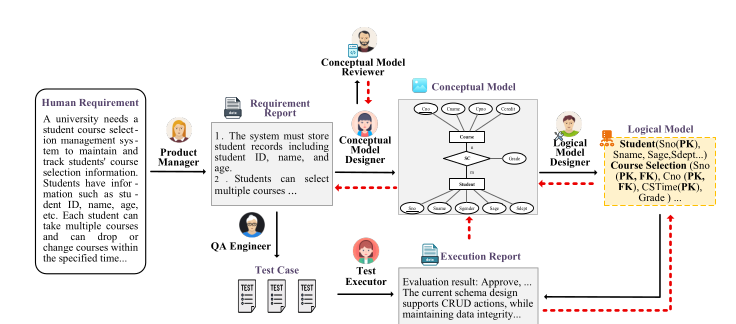
\includegraphics[width=0.85\linewidth]{images/ai/SchemaAgent.png}
  \caption{SchemaAgent Design}
  \label{fig:SchemaAgent}
\end{figure}

\subsection{Evaluation challenges in schema generation}
\label{sec:evaluation-challenges}

Evaluating automatically generated schemas presents conceptual and practical challenges that have been recognized across database, ontology, and conceptual-modelling literatures. Unlike query-generation tasks where execution provides an objective correctness signal, schema design admits multiple valid representations for the same requirements. Design choices such as surrogate versus natural keys, degree of normalization, whether to introduce associative entities, and denormalization for performance produce a \emph{space of acceptable schemas} rather than a single ground-truth. This multiplicity complicates the construction of canonical benchmarks and demands granular evaluation strategies.

The research community has therefore adopted mixed evaluation regimes. Component-level metrics (entity and attribute recall/precision, key detection rates, foreign-key recovery) enable objective comparisons of discrete aspects of schema proposals. Human expert assessments remain indispensable for judging global design quality, trade-offs, and workload-driven decisions. In addition, task-oriented evaluation (measuring how well generated schemas support downstream queries, analytics, or API needs) provides pragmatic evidence of utility even when structural mismatches exist between automatic outputs and a particular gold standard \cite{schemaagent2025,abedjan2016,yu2018spider}.

Recent benchmark creation efforts for requirement→schema tasks respond directly to these issues by decomposing evaluation into measurable components and by proposing adjudication procedures for cases where multiple semantically-equivalent schemas exist. Still, the literature acknowledges that no single automatic metric captures all aspects of design quality and that standardized protocols for multi-gold annotation, expert adjudication, and downstream task evaluation are necessary to enable reproducible research in Text\textrightarrow Schema \cite{schemaagent2025}.

Manually evaluating each schema is prohibitively time-consuming and makes it difficult to quantitatively assess model performance. Consequently, SchemaAgent introduces an automated evaluation approach using manually annotated schemas in RSchema as the ground truth. Each schema undergoes multiple rounds of evaluation to ensure correctness and quality. A schema consists of five key components: relation schema (table), attribute, primary key, foreign key, and constraint. The evaluation metrics include average F1 score and exact matching accuracy (Acc.) between predicted and ground truth values. Accuracy is set to 1 only if the F1 score equals 1; otherwise, it is 0.

\textbf{Relation schema (Table).} Since generative models may produce different tokens with similar meanings, three alignment methods are used to match predicted schema names with ground truth:
\begin{enumerate}
    \item \emph{Synonym Matching:} WordNet is used to extract synonyms of predicted values and verify inclusion of the ground-truth value.
    \item \emph{Similarity Matching:} all-MiniLM-L6-v2 measures semantic similarity with a threshold $\delta_0 = 0.6$.
    \item \emph{String Matching:} The longest common substring between predicted and ground-truth values is checked against $\delta_1 = 0.75$.
\end{enumerate}

For a schema with multiple tables, the table-level F1 score is computed as:
\begin{equation}
F1_{\text{table}} = 2 \times \frac{P \times R}{P + R}
\end{equation}
where
\begin{equation}
P = \frac{|R_{\text{gt}} \cap R_{\text{pred}}|}{|R_{\text{pred}}|}, \quad 
R = \frac{|R_{\text{gt}} \cap R_{\text{pred}}|}{|R_{\text{gt}}|}
\end{equation}
$R_{\text{gt}}$ is the set of relation schemas in the ground truth, and $R_{\text{pred}}$ is the predicted set. The average error rate of this metric is 1.8\%, demonstrating reliability compared with manual evaluation.

\textbf{Attributes.} The same three alignment methods are applied to attribute sets in matched tables. Attribute F1 is computed as:
\begin{equation}
F1_{\text{attrs}} = \frac{1}{|R_{\text{gt}}|} \sum_{R_{\text{gt},i} \in R_{\text{gt}}} F1_{\text{attrs}}(R_{\text{gt},i})
\end{equation}
where $F1_{\text{attrs}}(R_{\text{gt},i})$ compares the attributes of the $i$-th ground-truth table with the predicted table.

\textbf{Keys} Primary and foreign keys require exact matching, with Acc. set to 1 only when predicted and golden sets are identical. Data type accuracy is computed only for successfully matched attributes.

These metrics, combining semantic alignment and exact matching, enable automated, reproducible assessment of generated schemas. Manual evaluation of 20 randomly selected schemas (over 100 tables) confirms that automated metrics are consistent with expert judgment, providing a reliable quantitative signal for model performance.




\subsection{Synthesis and open directions}
\label{sec:open-directions}

Collectively, the prior literature indicates that Text\textrightarrow Schema is a challenging but tractable research direction that benefits from hybrid approaches. Core open problems include: (1) principled methods to infer functional dependencies from text or small-sample exemplars; (2) robust disambiguation strategies for cardinalities and participation constraints; (3) workload-aware normalization that integrates expected query patterns into design decisions; and (4) standardized evaluation frameworks that accommodate multiple valid schemas. Promising methodological building blocks include classical FD theory and instance-aware FD miners, semantic grounding via ontologies or schema corpora, and the new generation of LLM-based tools and multi-agent frameworks for hypothesis generation and verification \cite{bernstein1976,huhtala1999tane,navarro2009,parciak2024,schemaagent2025}.
